\subsection{Analisi preliminare, verifica delle leggi di Fresnel}\label{subsec:analisi-dati}
  In questo modo, abbiamo ottenuto le misure di intensità riflessa $I_\pi$ e $I_\sigma$ [fig ??]. Per ottenere i
  coefficienti di Fresnel, abbiamo normalizzato i dati ottenuti tenendo conto che:
  there is no difference between Rp and Rs at normal incidence
  at glancing angle in the less-dense medium the reflection coefficients are ±1,
  Come descritto in [Lipson]
  Da queste misure abbiamo ricavato anche l’angolo di Brewster, osservando per quale valore di $\theta_i$
  l’intensità $I_\pi$ si annulla.
  %TODO

  \begin{figure}[h]
    \centering
    \caption{Sburino}
    \begin{subfigure}{.4\textwidth}
      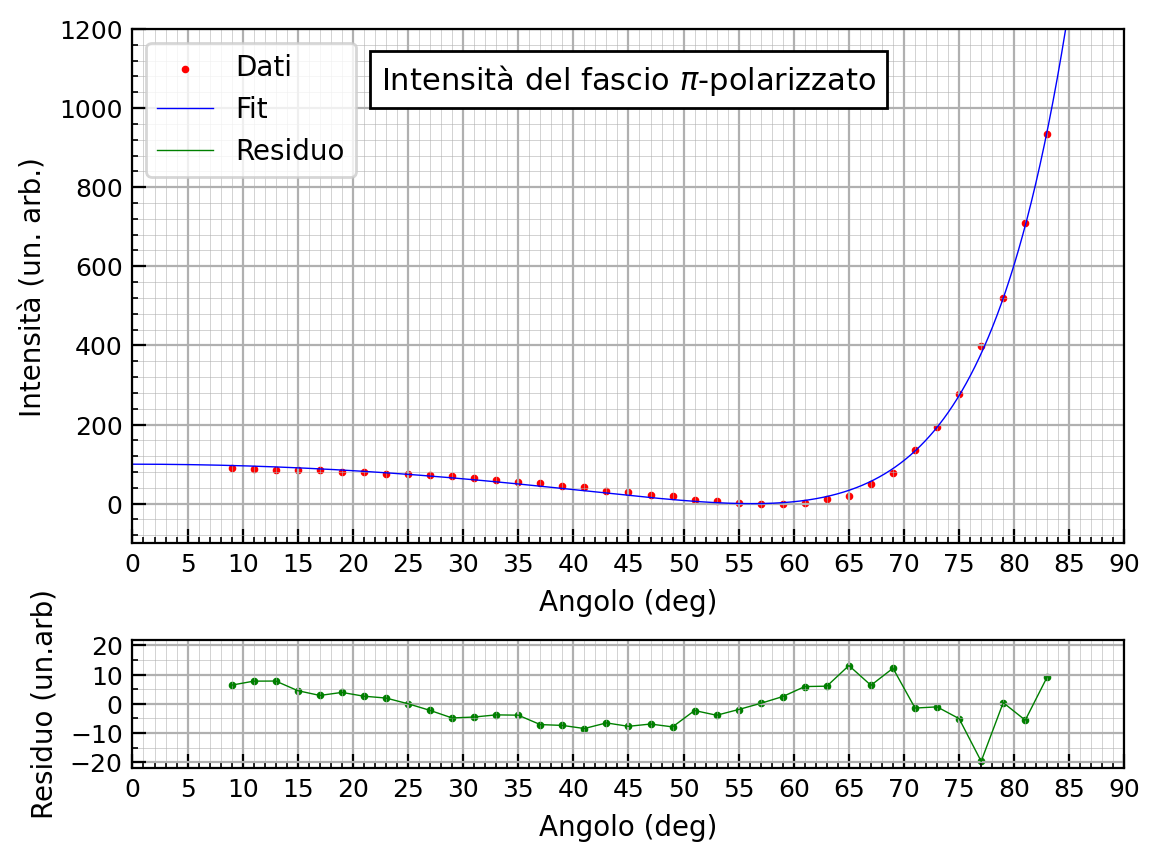
\includegraphics[width=7cm]{./graphs/raw-pi.png}
      \caption{
        \emph{
          sbüro
        }
      }
      \label{fig:raw-pi}
    \end{subfigure}%
    \hspace{20mm}
    \begin{subfigure}{.4\textwidth}
      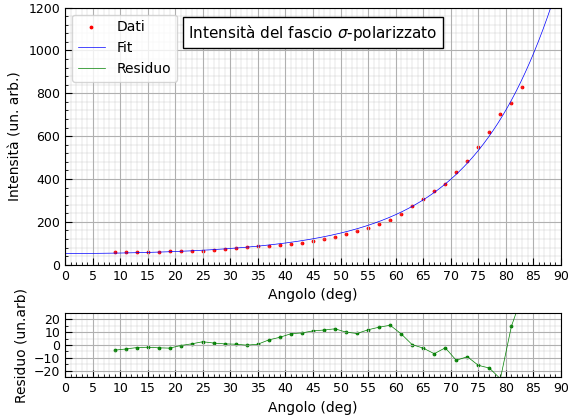
\includegraphics[width=7cm]{./graphs/raw-sigma.png}
      \caption{
        \emph{
          sbruña
        }
      }
      \label{fig:raw-sigma}
    \end{subfigure}
  \end{figure}
  %
  bla bla bla dopo questo abbiamo normalizzato i dati bla bla bla
  Donec ullamcorper, felis non sodales commodo, lectus velit ultricesaugue,adignissimnibhlectusplaceratpede. Vivamusnuncnunc,molestieut,ultriciesvel,semperin,velit. Ut porttitor. Praesent in sapien. Lorem ipsum dolor sit amet, consectetuer adipiscing elit. Duisfringilla tristique neque. Sed interdum libero ut metus. Pellente
  %
  \begin{figure}[h]
    \centering
    \caption{Smegma}
    \begin{subfigure}{.4\textwidth}
      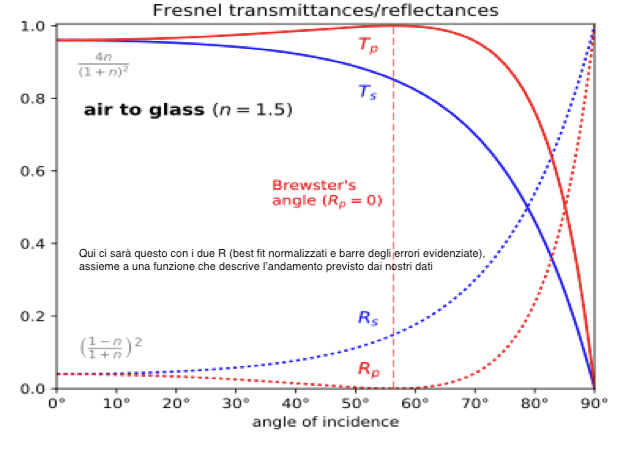
\includegraphics[width=7cm]{./graphs/normalised-coefficients.png}
      \caption{
        \emph{
          spregna
        }
      }
      \label{fig:normalised-coefficients}
    \end{subfigure}%
    \hspace{20mm}
    \begin{subfigure}{.4\textwidth}
      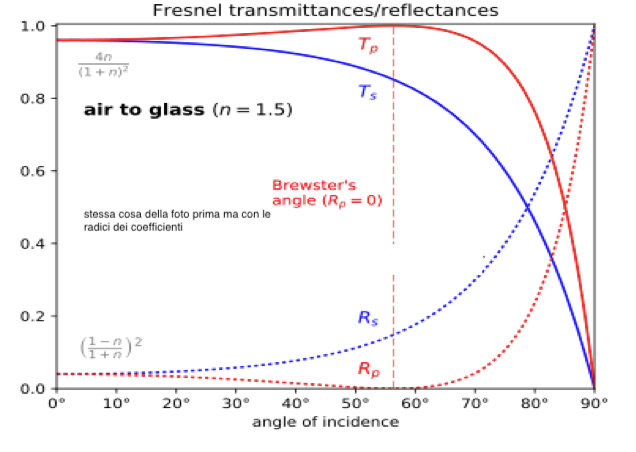
\includegraphics[width=7cm]{./graphs/amplitude-coefficients.png}
      \caption{
        \emph{
          bora
        }
      }
      \label{fig:raw-sigma}
    \end{subfigure}
  \end{figure}
  sì ceh insomma ok la roba fitta kek siamo molto bravi


\subsection{Misura dell'angolo di Brewster}\label{subsec:angolo-di-brewster}
  \blindtext[1]
  ciao
  %
  \begin{figure}[h]
    \centering
    \caption{brema}
    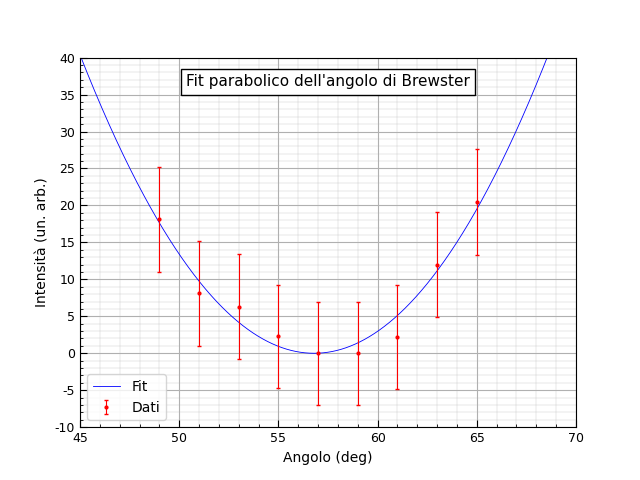
\includegraphics[width=7cm]{./graphs/brewsters-angle.png}
    \label{fig:brewsters-angel}
  \end{figure}
  % TODO
\endinput



